\documentclass{article}

\usepackage{imta_core}
\usepackage{imta_extra}
\usepackage{adjustbox}
\usepackage[backend=biber, sorting=none]{biblatex}
\usepackage[francais]{babel}
\usepackage{subfig}
\usepackage{scrextend}

\usepackage{csquotes}
\addbibresource{../common/bibliography.bib}

\author{Armand Foucault}
\date{Novembre 2017}
\title{Métamodélisation du langage B et \mbox{interactions} avec un prouveur B}
\subtitle{Plan de travail, rapport bibliographique}

% \imtaSetIMTStyle

% PACKAGES

\usepackage[francais]{babel} % Sehr wichtig: import this one first
\usepackage{imta_core}
\usepackage{imta_extra}
\usepackage{adjustbox}
\usepackage[backend=biber, sorting=none]{biblatex}
\usepackage{subfig}
\usepackage{scrextend}
\usepackage{pmboxdraw}
\usepackage{csquotes}
\usepackage{colortbl}


% BIBLIOGRAPHY

\addbibresource{../common/bibliography.bib}


% METAINFO

\author{Armand Foucault}
\date{Novembre 2017}
\title{Métamodélisation du langage B\\Intégration d'Event-B à OpenFlexo}
\subtitle{Projet S5 - Rapport technique}


% COMMANDS

\newcommand{\javacode}[1]{\imtaInlinecode{java}{#1}}
\newcommand{\rawHref}[1]{\hspace{0.2em}\textcolor{imtaLightBlue}{\href{#1}{#1}}\hspace{0.2em}}


% COLUMN TYPES

\newcolumntype{L}[1]{>{\raggedright\let\newline\\\arraybackslash\hspace{0pt}}m{#1}}
\newcolumntype{C}[1]{>{\centering\let\newline\\\arraybackslash\hspace{0pt}}m{#1}}
\newcolumntype{R}[1]{>{\raggedleft\let\newline\\\arraybackslash\hspace{0pt}}m{#1}}


% COLORS

\colorlet{Header}{imtaGreen}
\definecolor{Task}{RGB}{209, 231, 151}
\definecolor{Subtask}{RGB}{236, 245, 214}

% \colorlet{Header}{imtaLightBlue}
% \definecolor{Task}{RGB}{179, 242, 255}
% \definecolor{Subtask}{RGB}{230, 251, 255}


\newcommand{\rawHref}[1]{\hspace{0.2em}\textcolor{imtaLightBlue}{\href{#1}{#1}}\hspace{0.2em}}
\usepackage{colortbl}
\newcolumntype{L}[1]{>{\raggedright\let\newline\\\arraybackslash\hspace{0pt}}m{#1}}
\newcolumntype{C}[1]{>{\centering\let\newline\\\arraybackslash\hspace{0pt}}m{#1}}
\newcolumntype{R}[1]{>{\raggedleft\let\newline\\\arraybackslash\hspace{0pt}}m{#1}}
\colorlet{Header}{imtaGreen}
\definecolor{Task}{RGB}{209, 231, 151}
\definecolor{Subtask}{RGB}{236, 245, 214}
% \colorlet{Header}{imtaLightBlue}
% \definecolor{Task}{RGB}{179, 242, 255}
% \definecolor{Subtask}{RGB}{230, 251, 255}


%%%%%%%%%%%%%%%%%%%%%%%%%%%%%%% 
%%%%%%%%%% BEGINNING %%%%%%%%%% 
\begin{document}

\imtaMaketitlepage

\tableofcontents

\newpage

\chapter{Écriture d'un plugin pour Rodin}

Nous procédons dans un premier temps à l'implémentation d'un plugin élémentaire pour Rodin, dans le but de nous familiariser avec son API.
Pour ce faire, nous reprenons le tutoriel d'Aymerick Savary \cite{asavary}.
Ce tutoriel explique pas à pas le développement d'un plugin simple pour Eclipse, et vient y intégrer des appels à l'API de Rodin.

Nous construisons ensuite l'abstraction présentée au chapitre \ref{sec:apihandle}, et l'intégrons dans un projet \textit{plugin} Eclipse, %
qui disposera ainsi de fonctions simples d'utilisation pour manipuler les projets Rodin.
Nous présenterons au chapitre suivant la communication entre ce plugin et OpenFlexo.

Nous dirons que l'API de Rodin fonctionne en mode \textit{plugin}.
Ce mode est très confortable, car il laisse à Eclipse la charge d'initialiser les environnements nécessaires à la manipulation de projets Rodin.


\section{Implémentation d'un plugin élémentaire Rodin}

Nous nous proposons de réaliser un plugin élémentaire pour Rodin.
Nous commençons par écrire un plugin de base pour Eclipse, puis nous l'intégrons à Rodin, et enfin nous y ajoutons des appels à l'API de Rodin.

\subsection{Écriture d'un plugin générique Eclipse}

Nous commençons par télécharger le package d'Eclipse
\footnote{À l'heure de la rédaction de ce document, la liste de packages disponibles se trouve sur le site d'Eclipse, %
à l'adresse \href{https://www.eclipse.org/downloads/eclipse-packages/}{https://www.eclipse.org/downloads/eclipse-packages/}
} dédié au développement de RCP\footnote{Les applications client "riches"}.
Après installation, nous lançons Eclipse, et créons un nouveau projet \textit{via} le menu \textit{File > New > Plug-in Project}.
Nous appelons notre projet \textit{HelloWorldPlugin} (figure \ref{fig:newPlugin1}), cliquons deux fois sur \textit{Next} pour arriver %
sur la page de sélection du modèle de plugin (figure \ref{fig:newPlugin3}), et choisissons \textit{Hello, World Command} afin de voir la base d'un plugin.


\begin{figure}[H]
\centering
\subfloat[Création d'un nouveau plugin - 1/4]{{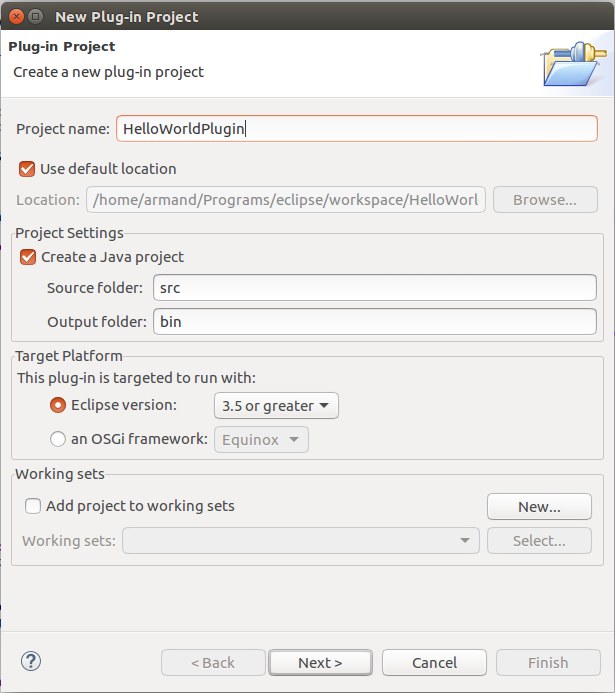
\includegraphics[width=0.4\linewidth]{pictures/newPlugin1.png}\label{fig:newPlugin1}}}%
    \qquad
\subfloat[Création d'un nouveau plugin - 2/4]{{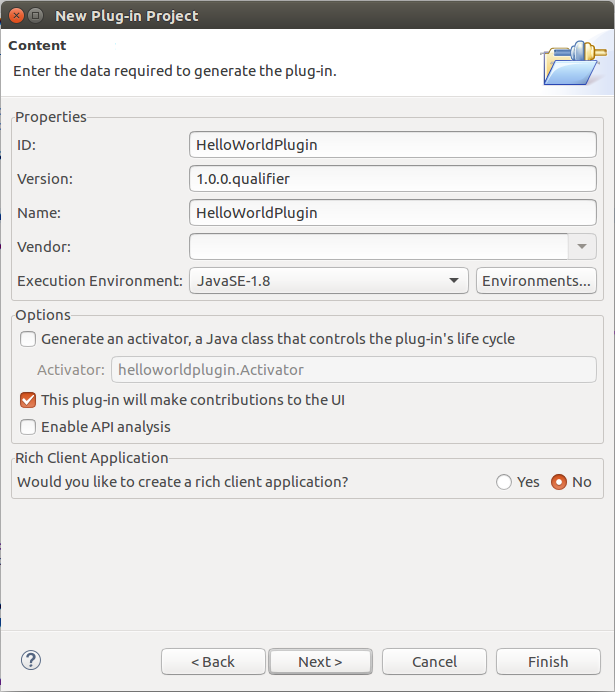
\includegraphics[width=0.4\linewidth]{pictures/newPlugin2.png}\label{fig:newPlugin2}}}%
    \vspace{0.5cm}
\subfloat[Création d'un nouveau plugin - 3/4]{{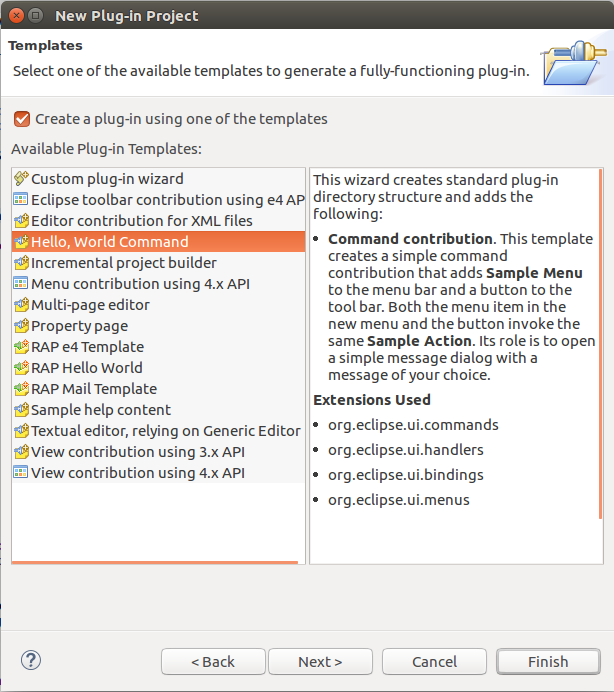
\includegraphics[width=0.4\linewidth]{pictures/newPlugin3.png}\label{fig:newPlugin3}}}%
    \qquad
\subfloat[Création d'un nouveau plugin - 4/4]{{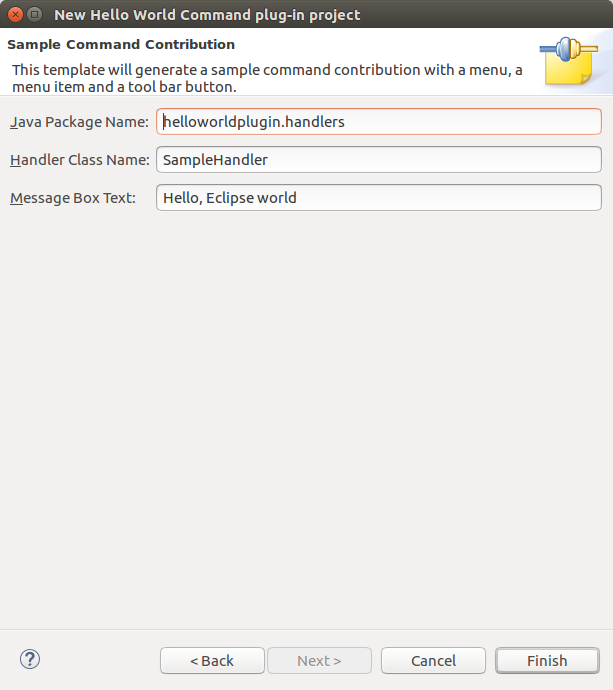
\includegraphics[width=0.4\linewidth]{pictures/newPlugin4.png}\label{fig:newPlugin4}}}%

\caption{Création d'un nouveau plugin dans Eclipse}
\end{figure}


La classe qui nous intéresse est \imtaInlinecode{java}{SampleHandler}, se trouvant dans \imtaInlinecode{text}{./src/helloworldplugin.handlers}.

\begin{imtaCode}{java}
public class SampleHandler extends AbstractHandler {

    @Override
    public Object execute(ExecutionEvent event) throws ExecutionException {
        IWorkbenchWindow window = HandlerUtil.getActiveWorkbenchWindowChecked(event);
            MessageDialog.openInformation(
                            window.getShell(),
                            "HelloWorldPlugin",
                            "Hello, Eclipse world");
            return null;
    }
}
\end{imtaCode}

Nous exécutons le plugin \textit{via} le menu \textit{Run > Run Configurations...}, où nous choisissons \textit{Eclipse Application}, sélectionnons \textit{org.eclipse.platform.ide} %
dans l'encadré \textit{Program to Run} sous l'option \textit{Run a product} (figure \ref{fig:runPlugin1}).
Enfin, nous cliquons sur \textit{Run}.
Une nouvelle instance d'Eclipse s'ouvre, avec un bouton supplémentaire correspondant à notre plugin.
Lorsque nous cliquons sur celui-ci, une fenêtre s'ouvre, affichant le message \textit{"Hello, Eclipse world"} (figure \ref{fig:runPlugin2}).

\begin{figure}[H]
    \centering

    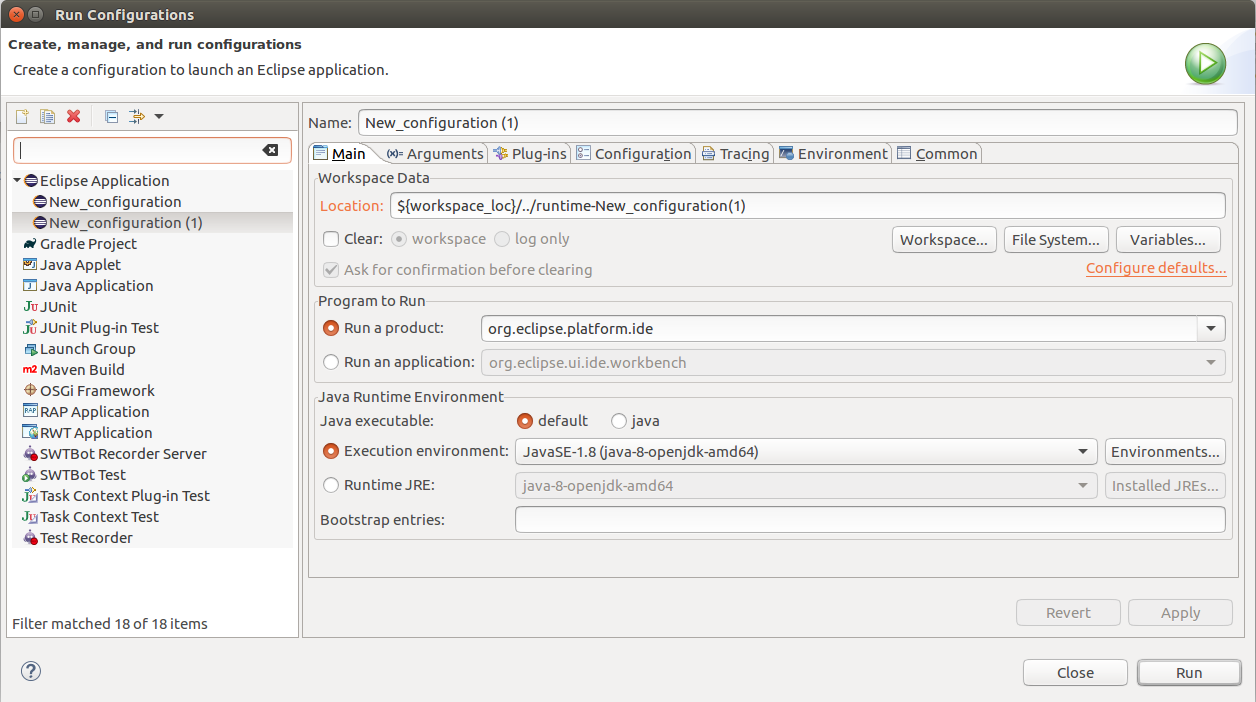
\includegraphics{pictures/runPlugin1.png}

    \caption{Exécution du plugin dans une nouvelle instance d'Eclipse - 1/2}
    \label{fig:runPlugin1}
\end{figure}

\begin{figure}[H]
    \centering

    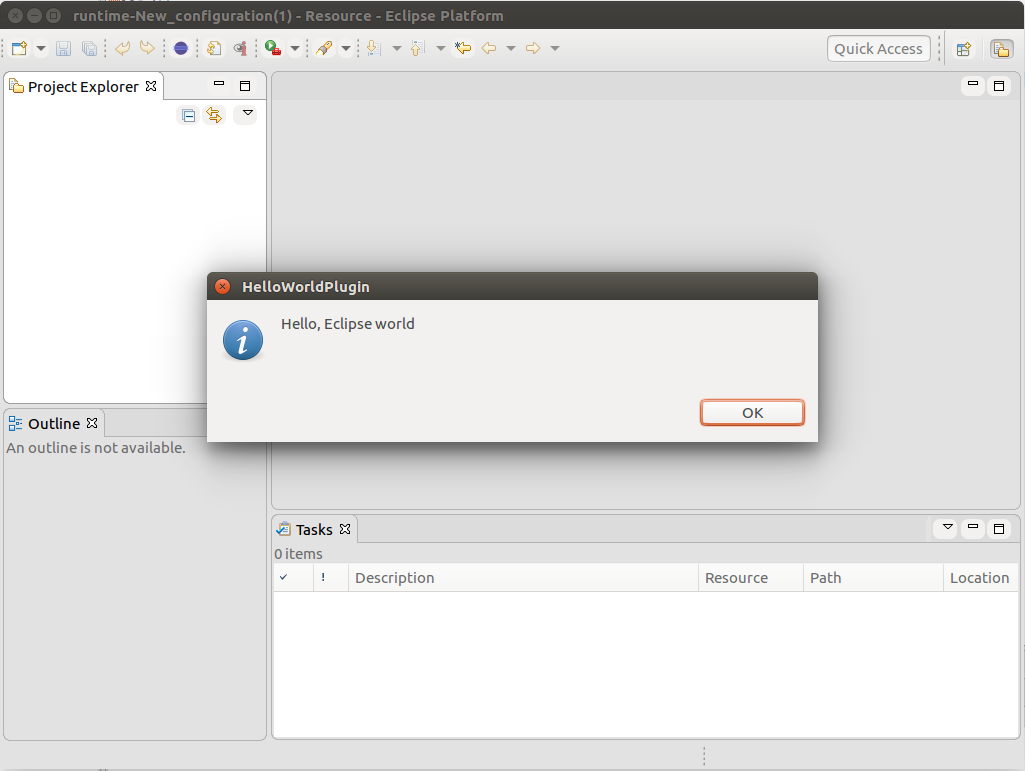
\includegraphics{pictures/runPlugin3.png}

    \caption{Exécution du plugin dans une nouvelle instance d'Eclipse - 2/2}
    \label{fig:runPlugin2}
\end{figure}


\subsection{Intégration dans Rodin}

Nous nous intéressons maintenant à l'intégration du plugin dans Rodin.
Nous téléchargeons tout d'abord Rodin\footnote{%
L'adresse du téléchargement est disponible sur le wiki Rodin : \href{http://wiki.event-b.org/index.php/Main\_Page}{http://wiki.event-b.org/index.php/Main\_Page}}.
Une fois Rodin installé, nous retournons dans notre éditeur Eclipse pour RCP, et choisissons Rodin comme plateforme d'exécution.
Dans le menu \textit{Run > Run Configurations...}, nous choisissons cette fois-ci \textit{org.rodinp.platform.product} comme produit à exécuter, %
puis cliquons sur \textit{Run} (figure \ref{fig:runPlugin3}).
Une instance de Rodin se lance alors, où nous pouvons créer une machine et interagir avec divers composants du monde Event-B, mais aussi %
invoquer notre plugin (figure \ref{fig:runPlugin4}).

\begin{figure}[H]
    \centering

    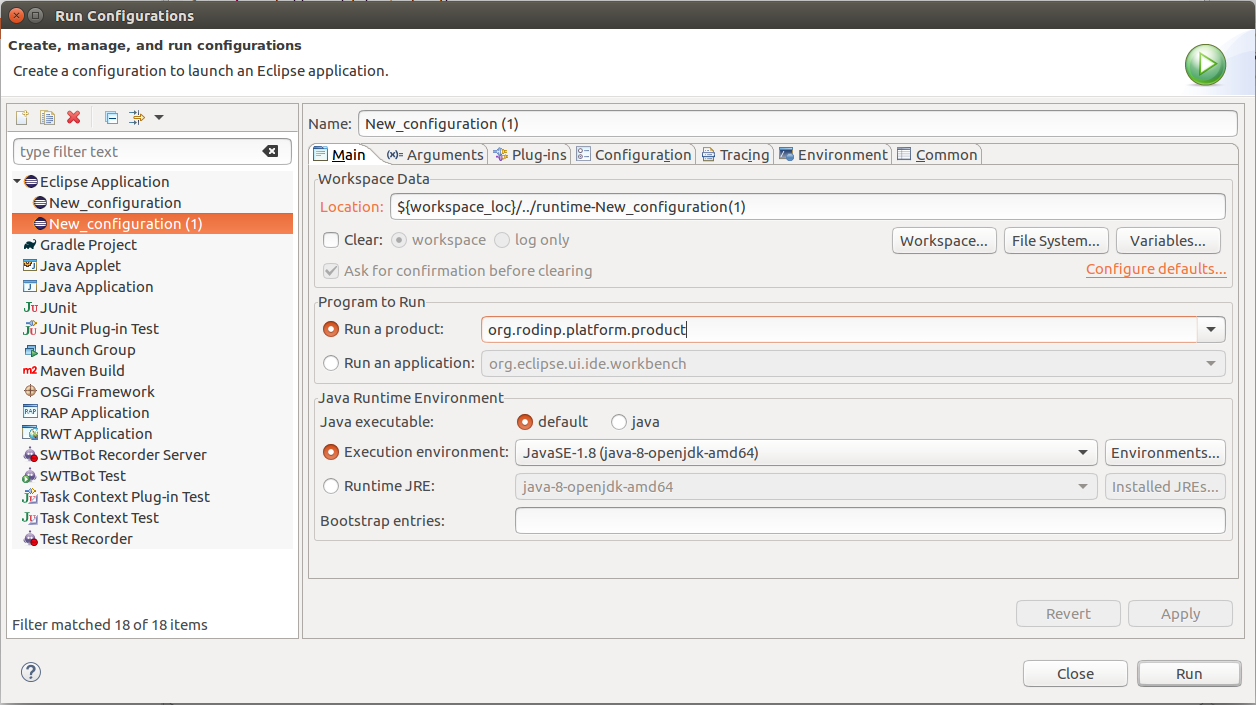
\includegraphics{pictures/runPlugin4.png}

    \caption{Exécution du plugin dans Rodin - 1/2}
    \label{fig:runPlugin3}
\end{figure}

\begin{figure}[H]
    \centering

    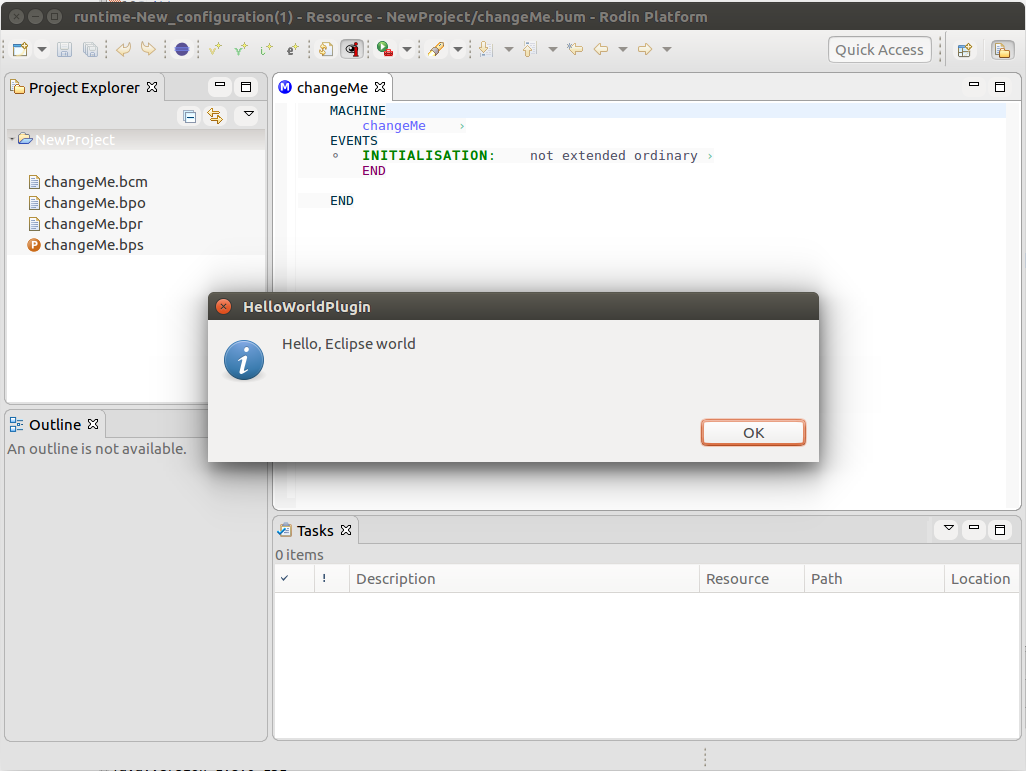
\includegraphics{pictures/runPlugin5.png}

    \caption{Exécution du plugin dans Rodin - 2/2}
    \label{fig:runPlugin4}
\end{figure}


\subsection{Appels à l'API de Rodin}

Nous souhaitons maintenant que notre plugin interagisse avec l'API de Rodin.
Nous ajoutons d'abord les packages nécessaires au manifeste, à savoir \imtaInlinecode{java}{org.eventb.core} et \imtaInlinecode{java}{org.rodinp.core}.
Nous ajoutons également \imtaInlinecode{java}{org.eclipse.core.runtime}, qui contient la classe \imtaInlinecode{java}{CoreException} dont hérite %
\imtaInlinecode{java}{RodinDBException}, levée par la plupart des méthodes utilisées, et qui doit être déclarée pour être attrapée.
Nous ouvrons donc le manifeste comme auparavant, cliquons sur l'onglet \textit{Dependencies}, et cliquons sur le bouton \textit{Add...}.
Nous obtenons une vue semblable à la figure \ref{fig:addDependencies1}, et après validation, l'encadré de dépendances comporte les packages indiqués en figure %
\ref{fig:addDependencies2}.

\begin{figure}[H]
    \centering

    \includegraphics{pictures/addDependencies1.png}

    \caption{Ajout des dépendances au manifeste}
    \label{fig:addDependencies1}
\end{figure}

\begin{figure}[H]
    \centering

    \fcolorbox{gray!50}{white}{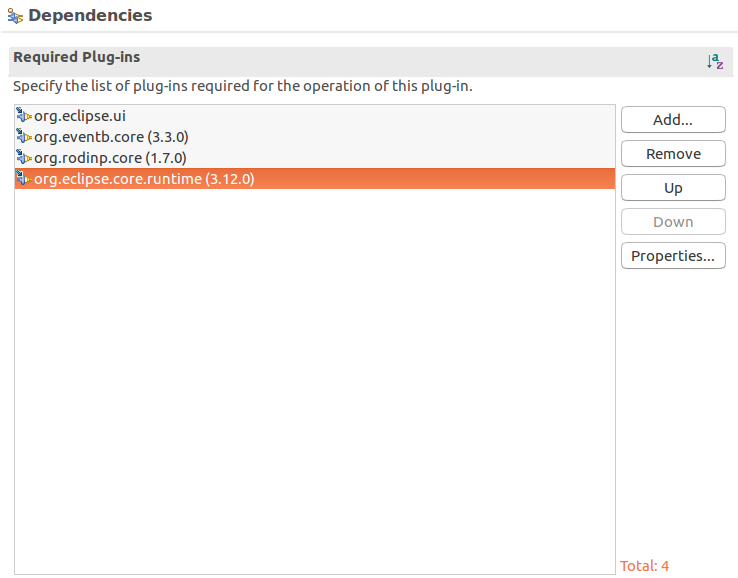
\includegraphics[width=0.6\linewidth]{pictures/addDependencies2.png}}

    \caption{Encadré des dépendances après import}
    \label{fig:addDependencies2}
\end{figure}

Nous créons dans la classe \imtaInlinecode{java}{SampleHandler} une méthode \imtaInlinecode{java}{listProjectElements}, listant les éléments d'un projet dont le nom %
est passé en paramètre.

\begin{imtaCode}{java}
public void listProjectElements(String projectName)
{
    IRodinProject project = RodinCore.getRodinDB().getRodinProject(projectName);
        try
        {
            for (IRodinElement element : project.getChildren())
            {
                if (element instanceof IRodinFile)
                {
                    IInternalElement root = ((IRodinFile) element).getRoot();
                    if (root instanceof IMachineRoot)
                    {
                        for (IInvariant invariant : 
                             ((IMachineRoot) root).getInvariants())
                        {
                            if (invariant.isTheorem())
                            {
                                System.out.println(
                                    "Théorème : " + invariant.getLabel() + " : "
                                    + invariant.getPredicateString());
                            }
                            else
                            {
                                System.out.println(
                                    "Invariant : " + invariant.getLabel() + " : "
                                    + invariant.getPredicateString());
                            }
                        }
                        for (IEvent event : ((IMachineRoot) root).getEvents())
                        {
                            System.out.println("Événement : " + event.getLabel());
                            for (IGuard garde : event.getGuards())
                            {
                                System.out.println(
                                    "Garde : " + garde.getLabel() + " : " 
                                    + garde.getPredicateString());
                            }
                        }
                    }
                }
            }
        } catch (RodinDBException e) {
        e.printStackTrace();
    }
}
\end{imtaCode}

Nous ajoutons un appel à cette méthode dans la méthode principale \imtaInlinecode{java}{SampleHandler.execute}, sur un projet Rodin nommé \imtaInlinecode{java}{"TestProject"}, %
que nous créons et remplissons d'éléments de test, comme en figure \ref{fig:rodinTestProject}.
Enfin, dans la console de l'instance de développement d'Eclipse, nous lisons les éléments listés comme montré en figure \ref{fig:rodinPluginConsole}.

\begin{figure}[H]
    \centering

    \begin{minipage}{.4\linewidth}
        \fbox{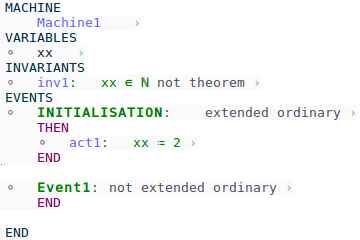
\includegraphics{pictures/rodinTestProject.png}}
        \caption{Machine de test dans Rodin}
        \label{fig:rodinTestProject}
    \end{minipage}%
    \qquad\qquad%
    \begin{minipage}{.4\linewidth}
        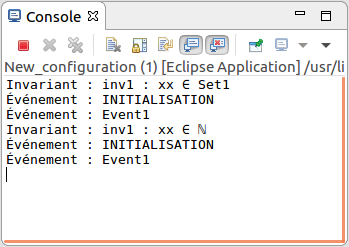
\includegraphics{pictures/rodinPluginConsole.png}
        \caption{Sortie dans la console d'Eclipse}
        \label{fig:rodinPluginConsole}
    \end{minipage}
\end{figure}

Nous pouvons pousser le développement du plugin de test, afin d'afficher les informations précédentes directement dans Rodin, c'est-à-dire dans l'environnement cible.
En reprenant la fenêtre de démonstration du plugin \textit{Hello, World}, nous obtenons la vue présentée en figure \ref{fig:rodinPluginWindow}.

\begin{figure}[H]
    \centering
    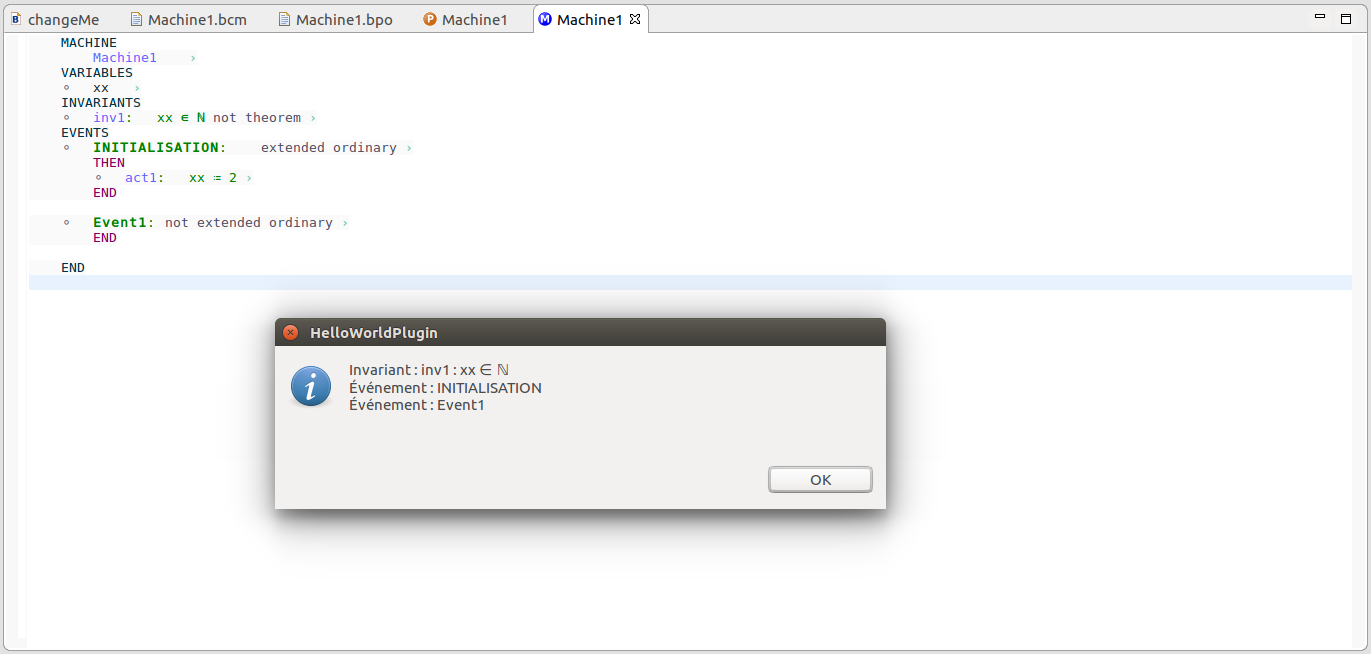
\includegraphics{pictures/rodinPluginWindow.png}
    \caption{Vue de Rodin avec la fenêtre d'informations du plugin}
    \label{fig:rodinPluginWindow}
\end{figure}

Maintenant que nous disposons d'un plugin de base, nous pouvons revenir à notre projet \textit{BlangFlexo} pour implémenter le package \javacode{org.blangflexo.plugin}, afin %
de réaliser la communication désirée.


\section{Communiquer avec OpenFlexo~: le package \texttt{org.blangflexo.plugin}}

% TODO: expliquer rapidement

\subsection{Point d'entrée du plugin}

L'exécution du plugin commence au moment où l'utilisateur appuie sur le bouton ajouté à la barre d'outils de Rodin.
Le \textit{handler} principal du plugin a pour seule fonction de démarrer l'écoute d'instructions, à travers la classe \javacode{InstructionListener} que nous présentons à la section suivante.

\begin{imtaCode}{java}
public class BlangFlexoHandler extends AbstractHandler {
    
    
    @Override
    public Object execute(ExecutionEvent event) throws ExecutionException {
        if (!ApiAbstractor.isStarted())
        	ApiAbstractor.start();
        
        new InstructionListener(20001).start();
        return null;
    }
}
\end{imtaCode}

\subsection{Implémentation d'un serveur TCP}

Nous souhaitons que notre plugin écoute sur une socket TCP les instructions envoyées par OpenFlexo.
Nous implémentons donc un serveur TCP, et OpenFlexo lui enverra ses commandes en mode client.

Le serveur TCP est implémenté par la classe \javacode{org.blangflexo.plugin.InstructionListener}.
Son fonctionnement est volontairement simple~: il attend une connexion sur le port \texttt{20001}, et une fois une connexion acceptée, attend une instruction et l'exécute.
Il renvoie enfin un message indiquant si l'instruction s'est exécutée correctement.

Le serveur est implémenté sous la forme d'un thread, afin de ne pas interférer avec le thread principal d'Eclipse.
Son cycle de vie est implémenté par la méthode \javacode{InstructionListener.run} que nous présentons ici.
La gestion des erreurs et de la fermeture propre de la socket a volontairement été cachée dans le code qui suit pour des raisons de lisibilité, mais est naturellement %
présente dans le code.

\begin{imtaCode}{java}
public void run() {
    String instruction;
    String response;
    ServerSocket socket;
    BufferedReader inFromClient;
    DataOutputStream outToClient;
    
    // Ouverture de la socket d'écoute sur 'port', attribut d'instance
    socket = new ServerSocket(port);
    
    // Acceptation de la connexion cliente
    Socket connectionSocket = socket.accept();
    
    // Création des canaux de communication
    inFromClient = new BufferedReader(new InputStreamReader(connectionSocket.getInputStream()));
    outToClient = new DataOutputStream(connectionSocket.getOutputStream());
    
    // REPL
    while (true) {
        instruction = inFromClient.readLine();
        boolean success = ApiOperationDispatcher.execute(instruction);
        response = success ? "Success" : "Failure";
        outToClient.writeBytes(response);
    }
}
\end{imtaCode}

Les messages reçus par le serveur sont transmis à la classe \javacode{ApiOperationDispatcher}, qui se charge de les interpréter en tant qu'instructions, et de les exécuter.

\subsection{Exécution des instructions}

\newpage
%\section{Développement d'un Technology Adapter Rodin}

\subsection{Étude de la documentation de l'API Rodin}

\subsection{Architecture du Technology Adapter}

\subsection{Réalisation du Technology Adapter}

\subsubsection{Création d'un projet Rodin}

Dépendances : org.eclipse.core.resources

Le wiki Rodin fournit une solution permettant de créer dynamiquement et programmatiquement des projets, \textit{via} l'API.
Nous réutilisons ce code, et l'intégrons au plugin de test sous la forme d'une méthode \imtaInlinecode{java}{createRodinProject}.



Dépendances

\begin{itemize}
    \item org.eclipse.core.resources
    \item org.eclipse.core.runtime
    \item org.eclipse.equinox.common
    \item org.eclipse.equinox.registry
    \item org.eventb.core
    \item org.rodinp.core
\end{itemize}

%\newpage
\chapter{Étude de l'API Rodin}

\section{Éléments de machines Event-B}

L'API de Rodin définit, dans les packages préfixés par \javacode{org.eventb.}, les éléments relatifs à la description de systèmes %
avec la méthode Event-B.
Elle définit d'une part les protocoles de ces éléments sous la forme d'interfaces, et leur implémentation en tant que classes.
Dans cette section, nous présentons d'abord les protocoles implémentés par les éléments de la méthode Event-B, puis les classes qui leur font écho.

\subsection{Protocoles}

L'API de Rodin définit, dans le package \javacode{org.eventb.core}, les protocoles que chacun des types d'éléments %
d'une machine B doit respecter.
Comme le cœur de Rodin est écrit en Java, il est naturel que ces protocoles soient des interfaces.
Nous avons donc, pour chaque type d'élément Event-B, le contrat à respecter, représenté par une interface.
Nous retrouvons ainsi les interfaces \javacode{IAction}, \javacode{IEvent}, \javacode{IInvariant}...
Nous nous proposons de présenter, à titre d'exemple mais aussi pour approfondir notre compréhension de l'API, l'interface \javacode{IEvent}.

\subsubsection{Un exemple : \texttt{IEvent}}

L'interface \javacode{IEvent} présente principalement des accesseurs, permettant d'accéder aux sous-éléments d'un évènement Event-B.
Ces éléments sont les suivants~:

\begin{itemize}
    \item Les actions \javacode{IAction};
    \item Les gardes, implémentant \javacode{IGuard};
    \item Les variables locales, implémentant \javacode{IVariable};
    \item Les clauses de raffinement, implémentant \javacode{IRefinesEvent};
    \item Les témoins, implémentant \javacode{IWitness};
\end{itemize}

L'interface \javacode{IEvent} impose donc l'existence d'accesseurs à ces sous-éléments.
Ces accesseurs sont de deux types : nommé, et exhaustif.

Les accesseurs nommés permettent d'accéder à un sous-élément par son nom.
Ainsi, la méthode \javacode{getGuard} prend un \javacode{String} en argument, et renvoie une instance de \javacode{IGuard}, portant le nom spécifié.
Cette instance peut ne pas exister dans l'instance d'\javacode{IEvent}.
Cela signifie que la méthode \javacode{getGuard} renvoie systématiquement une garde portant le nom demandé, mais que celle-ci %
peut ne pas être attachée à l'évènement concerné.

Les accesseurs exhaustifs, quant à eux, renvoient la liste des sous-éléments de l'élément concernés.
Ainsi, la méthode \javacode{getActions} ne prend aucun argument, et renvoie un tableau de type \javacode{IActions[]}, dont nous savons que tous %
les éléments sont effectivement rattachés à l'évènement.

L'interface \javacode{IEvent} présente finalement les accesseurs suivants~:

\begin{itemize}
    \item \javacode{IAction getAction(String name)} et \javacode{IAction[] getActions()}
    \item \javacode{IGuard getGuard(String name)} et \javacode{IGuard[] getGuards()}
    \item \javacode{IParameter getParameter(String name)} et \javacode{IParameter[] getParameters()}
    \item \javacode{IRefinesEvent getRefinesClause(String name)} et \javacode{IRefinesEvent[] getRefinesClauses()}
    \item \javacode{IWitness getWitness(String name)} et \javacode{IWitness[] getWitnesses()}
\end{itemize}

Nous notons que les variables locales se retrouvent sous le nom de \javacode{Parameter}.

\subsubsection{Généralisation avec \texttt{IInternalElement}}

Les protocoles d'élément Event-B dérivent de la super-interface \javacode{IInternalElement}.
Cette interface permet entre autres de manipuler plus génériquement les sous-éléments des éléments Event-B.
Ainsi, les accesseurs nommés spécialisés tels que \javacode{getAction(String name)} ou \javacode{getInvariant(String name)} sont généralisés par %
la méthode \javacode{getInternalElement}, qui prend en paramètres le type de l'élément auquel accéder, et son nom.
Le type est défini comme une instance de \javacode{IInternalElementType<T extends IInternalElement>}, %
% ce qui permet de travailler avec des éléments de type indéterminé, en lui passant une instance de \javacode{IInternalElementType<IInternalElement>}.
sachant que les interfaces d'élément Event-B définissent chacune leur type à travers une variable statique \javacode{ELEMENT_TYPE}, instance de %
\javacode{IInternalElementType<T>} où \javacode{T} est l'interface elle-même.


\subsection{Implémentation}

L'implémentation des éléments Event-B et des interfaces du packages \javacode{org.eventb.core} est réalisée par les classes contenues dans %
le package \javacode{org.eventb.core.basis}.
Ainsi, chaque protocole défini dans le package \javacode{org.eventb.core} trouve sa réalisation, comme \javacode{IAction} implémentée par %
\javacode{Action}, ou encore \javacode{IGuard} implémentée par \javacode{Guard}.

Les implémentations de ces interfaces ne sont toutefois pas destinées à être utilisées telles quelles.
La documentation suggère en effet aux clients de l'API de ne manipuler que des instances des interfaces, ou bien à étendre les implémentations.
En reprenant l'exemple de l'élément \javacode{Event}, cela revient à ne travailler qu'avec des \javacode{IEvent}, ou alors à créer une classe fille de \javacode{Event}


\section{Éléments de projet Rodin}

L'API de Rodin fournit une surcouche aux éléments Event-B pour les manipuler en tant qu'éléments d'un projet Rodin, c'est-à-dire d'un type de projet Eclipse.
Les interfaces et classes auxquelles nous nous intéresseons sont ainsi définies dans le package \javacode{org.rodinp.core}.

\subsection{La base de données Rodin}

Nous nous proposons tout d'abord de présenter le cœur de Rodin : la base de données Rodin.
Implémentée par la classe \javacode{RodinDB}, celle-ci est chargée de conserver en mémoire les éléments de projets créés.
Toute manipulation d'élément de projet Rodin entraîne une écriture dans la base de données.
Par ailleurs, cette classe implémente un singleton, en lançant une exception de type \javacode{java.lang.Error} si son constructeur est appelée deux fois.

La classe \javacode{RodinDB} propose différentes méthodes de manipulation de projet, notamment \javacode{getWorkspace} et \javacode{getRodinProject}.
Elle est par ailleurs gérée par la classe \javacode{RodinDBManager}, qui la rend disponible à travers sa méthode \javacode{getRodinDB}.


\subsection{Protocole}

Le package \javacode{org.rodinp.core} définit tout d'abord le protocole des élément de projet Rodin, à travers l'interface \javacode{IRodinElement}.
Cette interface permet notamment d'interagir avec la base de données Rodin, avec la méthode \javacode{exists}, vérifiant si l'élément existe dans la base.
Elle permet également d'observer la hiérarchie d'éléments, à travers les méthodes \javacode{getAncestor} et \javacode{getParent}.

Par ailleurs, l'interface \javacode{IRodinElement} fournit également des méthodes de manipulation générique des éléments, telles que \javacode{getElementName} et %
\javacode{getElementType}.


\subsection{Implémentation}\label{sec:rodinProjectElementProtocol}

L'implémentation des éléments de projet Rodin et de l'interface \javacode{IRodinElement} est réalisée par la classe \javacode{RodinElement}.

En plus des principales méthodes que nous avons évoquées en section \ref{sec:rodinProjectElementProtocol}, la classe \javacode{RodinElement} fournit %
des accesseurs supplémentaires, dont \javacode{getChildren} et \javacode{getChildrenOfType}, renvoyant chacun une séquence d'éléments fils de l'élément courant.


\section{Résumé : l'exemple de la classe \texttt{Event}}

Nous résumons dans cette section les fonctionnalités d'une classe implémentant un élément Event-B.
Pour rester dans la même continuité, nous nous intéressons à l'implémentation d'un évènement, à travers la classe \javacode{Event}.
Nous présentons donc les méthodes qu'elle met à notre disposition, ainsi que les classes et interfaces dont elle les tient.

La figure suivante présente l'arbre d'héritage de la classe \javacode{Event}, annoté des interfaces implémentées par chacune des classes.

\begin{figure}[H]
\centering
\begin{imtaConsole}
java.lang.Object
│
└── org.eclipse.core.runtime.PlatformObject
    │
    └── org.rodinp.core.basis.RodinElement              -> IRodinElement
        │
        └── org.rodinp.core.basis.InternalElement       -> IInternalElement, IParent,
            │                                              IElementManipulation
            └── org.eventb.core.basis.EventBElement
                │
                └── org.eventb.core.basis.Event         -> IEvent
\end{imtaConsole}
\caption{Arbre d'héritage annoté de la classe \texttt{Event}}
\label{fig:inheritanceTreeEvent}
\end{figure}

Soit une instance de la classe \javacode{Event}, que nous nommons \javacode{event}.

À travers l'interface \javacode{IEvent}, nous pouvons utiliser les méthodes \javacode{event.getActions}, \javacode{event.getGuards}, \javacode{event.getParameters}, %
\javacode{event.getRefinesClauses}, et \javacode{event.getWitnesses}, ainsi que leurs pendants nommés, pour accéder respectivement aux actions, aux gardes, aux variables locales, %
aux clauses de raffinement, et aux témoins de l'évènement \javacode{event}.

Les méthodes héritées de \javacode{EventBElement} permettent de manipuler \javacode{event} comme un élément de projet Event-B.
Nous pouvons ainsi décider qu'\javacode{event} est un théorème avec \javacode{event.setTheorem}, obtenir le commentaire qui lui est associé avec \javacode{event.getComment}, %
et obtenir son nom et son expression \textit{via} les méthodes \javacode{event.getIdentifierString} et \javacode{event.getExpressionString}.

L'interface \javacode{IInternalElement} rapproche \javacode{event} de Rodin, en lui ajoutant des méthodes agissant sur la base de données Rodin.
Ainsi, nous pouvons forcer la création d'\javacode{event} dans cette dernière avec \javacode{event.create}, et lui attribuer un fils avec \javacode{event.createChild}.
Nous pouvons également comparer \javacode{event} à un autre élément, avec \javacode{event.hasSameAttributes}, ou encore \javacode{event.hasSameChildren}.
Nous pouvons par ailleurs interagir avec l'environnement de travail, et notamment récupérer le fichier courant avec \javacode{event.getRodinFile}.


\newpage

\nocite{*}

\printbibheading[title=Références, heading=bibintoc]

\printbibliography[keyword=bmethod, heading=subbibintoc, title={Méthode B}]

\printbibliography[keyword=rodin, heading=subbibintoc, title={Rodin}]

\printbibliography[keyword=openflexo, heading=subbibintoc, title={OpenFlexo}]


\end{document}
%%%%%%%%%% END %%%%%%%%%% 
%%%%%%%%%%%%%%%%%%%%%%%%% 
